\section{Разработка архитектуры наземной станции}
Аппаратная часть наземной станции состоит из:

--- компьютера;

--- передающего модуля радиоуправления;

--- видеоприемника;

--- устройства приема-передачи телеметрии.

Наземная станция должна обмениваться телеметрией с квадрокоптером, получать видеопоток с квадрокоптера, и отправлять управляющий сигнал в виде команд MAVROS. Чем больше бод -- рейт подключенных модулей и меньше задержка сигнала, тем быстрее осуществляется выполнение команд. Для устройств приема-передачи телеметрии рекомендуется бод -- рейт, равный 921600. Учитывая эти факторы, выбираются устройства телеметрии и видеоприемник.
К компьютеру по UART порту подключается модуль радиоуправления и устройство приема-передачи телеметрии. Через USB порт подключается видеоприемник. Настраиваем видеоприемник на диапазон частот, соответствующий частотам видеопередатчика квадрокоптера и переходим к программной части.

Для позиционирования робототехнических систем с помощью компьютерного зрения используются aruco маркеры -- квадратные маркеры, состоящий из широкой черной границы и внутренней двоичной матрицы, которая определяет его идентификатор (id). Черная рамка облегчает ее быстрое обнаружение на изображении, а двоичная кодификация позволяет ее идентифицировать \cite{opencv}.

В ходе исследования был найден пакет aruco\_pose, предназначенный для работы с aruco-маркерами. Для распознавания маркеров разработан aruco-detect. Они входят в образ clover, который предоставляет пакеты и инструменты для позиционирования и управления квадрокоптером на базе ROS по MAVROS. Образ clover подходит для выполнения поставленной задачи.

Программная часть представляет собой совокупность взаимодействущего программного обеспечения, включающего в себя:

--- операционную систему на базе ядра linux;

--- пакет clover;

--- qgroundcontrol.

В qgroundcontrol выставляется бод -- рейт. Далее происходит подключение и обмен данными с устройством приема-передачи телеметрии, расположенного на борту квадрокоптера.
По MAVLink протоколу передаются данные в указанный UART, и все программы, прослушивающие этот UART, порт имеют доступ к данным с борта квадрокоптера. Для взаимодействия через ROS инструменты необходима настройка всех параметров подключения. На данном этапе НИР используется готовой решение от Copter Express -- пакет clover, позволяющий производить настройку максимально просто. В launch файлах пакета прописываются все параметры. Указываем UART, бауд -- рейт, и в консоли запускаем clover с помощью команд:
\begin{MyCode}
	gs@groundstation:~$ source /home/clover/catkin\_ws/devel/setup.bash
	gs@groundstation:~$ roslaunch clover clover.launch
\end{MyCode}

После этого доступны все инструменты clover. На листинге \ref{lst:5} приведен результат выполнения команды для получения телеметрии. "frame\_id: ''" означает, что показания берутся в системе координат относительно квадрокоптера.
\begin{Program}[H]
	\caption{Вывод телеметрии квадрокоптера в консоли} \label{lst:5}
	\begin{MyCode}
		gs@groundstation:~$ rosservice call /get_telemetry "frame_id: ''" 
		frame_id: "map"
		connected: True
		armed: False
		mode: "MANUAL"
		x: -0.00260298536159
		y: -6.72723326716e-05
		z: 0.00103790743742
		lat: 0.0
		lon: 0.0
		alt: 0.0
		vx: -0.00717502878979
		vy: -0.00176917202771
		vz: 0.00364218326285
		pitch: 0.0221049506217
		roll: -0.0172985047102
		yaw: 0.000302107335301
		pitch_rate: 0.00245076417923
		roll_rate: 0.00449034944177
		yaw_rate: 0.00266480189748
		voltage: 12.1499996185
		cell_voltage: 4.05000019073
		gs@groundstation:~$
	\end{MyCode}
\end{Program}

Видеоприемник подключен в порт /dev/video0. Указываем его в launch-файле, перезагружаем clover и проверяем в web-браузере топики по адресу localhost:8080 (рис. \ref{fig:topic}).

\begin{figure}[H]
	\centering
	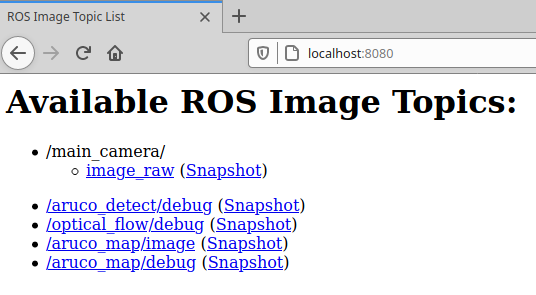
\includegraphics[width=0.5\linewidth]{../RW/pics/topic}
	\caption{Список топиков, доступный по умолчанию
	}
	\label{fig:topic}
\end{figure}

Список НОД также меняется в launch файлах. В image raw топике будет отображаться видеопоток, полученный видеоприемником с борта квадрокоптера, в остальных топиках публикуются:

--- aruco-detect (на image raw определяются с помощью openCV aruco маркеры);

--- optical flow (на изображение с image raw накладывается точка отсчета для лазерного дальномера);

--- aruco map (карта маркеров, прописанная в конфигурационном файле).

Optical flow отключаем, так как на БПЛА не установлен лазерный дальномер.